\chapter{Foundation}

In vessel handling terminology, maneuvering refers to the task of controlling a vessel’s movement using its propulsion and navigation systems; taking into account environmental forces such as wind, waves and, current acting on the vessel. Vessels move in a variety of marine environments. Starting from ports in harbors where the water is shallow and vessel traffic is high, a vessel might navigate the vast open seas to a different port in a harbour across the ocean. Vessels also navigate inland waterways such as rivers, canals, backwaters and creeks. More recently, developments in offshore wind farming and the oil and gas industry have necessitated regular and frequent visits to offshore structures located on continental shelves. Figure \ref{fig:northseamap} shows some prominent offshore oil fields in the North sea. 

%\begin{figure}
%	\centering
%	\begin{subfigure}{0.4\linewidth}
%		\centering
%		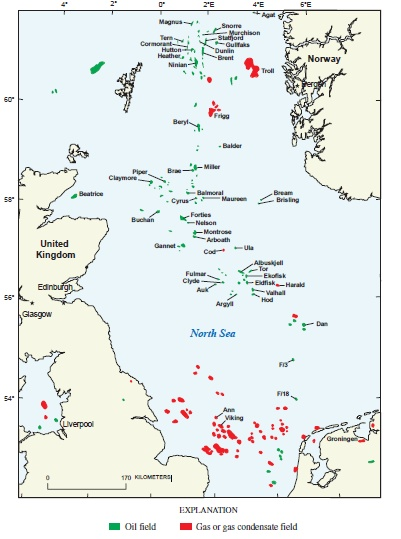
\includegraphics[scale=0.5]{northseaoilandgasmap}
%		\caption{Map of oil and gas fields in the North sea}
%		\label{fig:northseamap}
%	\end{subfigure}
%	\begin{subfigure}{0.4\linewidth}
%		\centering
%		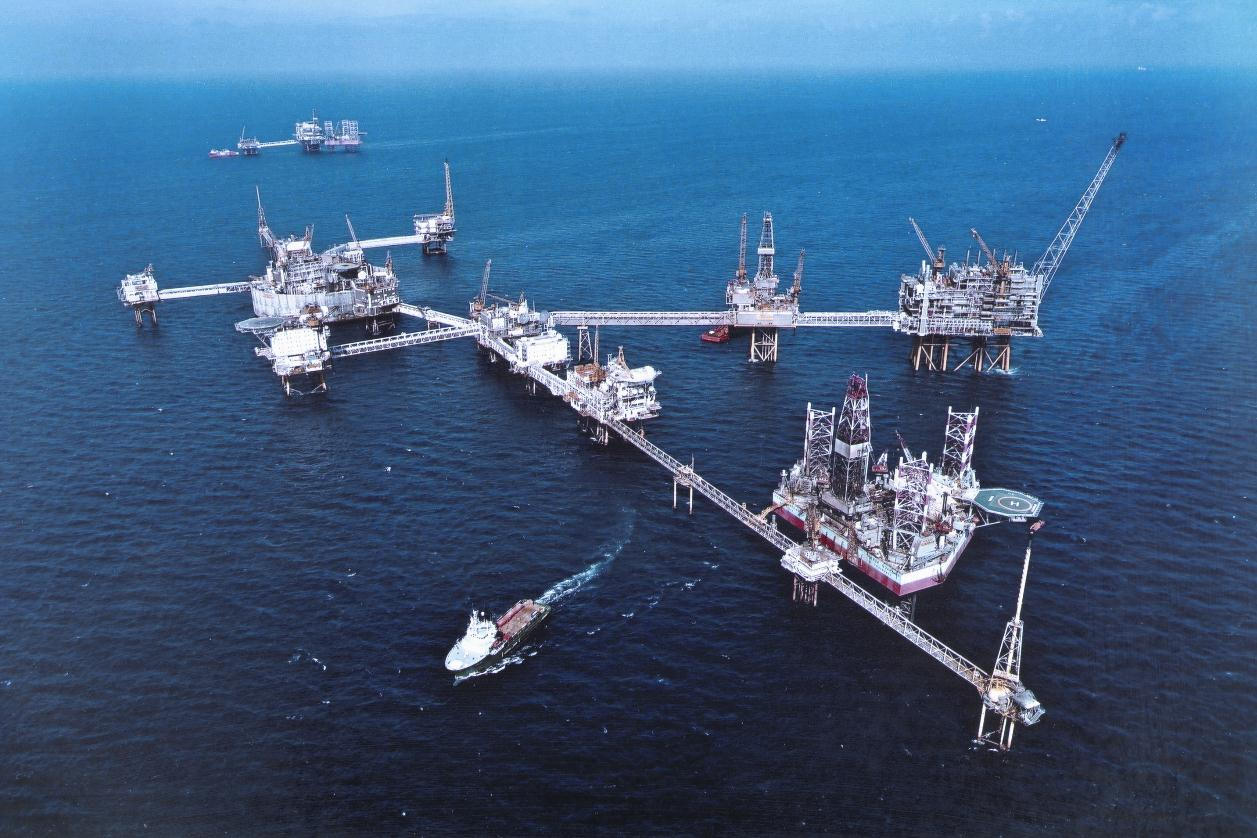
\includegraphics[scale=0.25]{ekofisk}
%		\caption{Ekofisk oil field in the Norwegian sector of the North Sea}
%		\label{fig:ekofisk}
%	\end{subfigure}
%	\caption{Offshore oil and gas fields in the North sea}
%	\label{fig:northseaoilandgas}
%\end{figure}

\begin{figure}
	\centering
	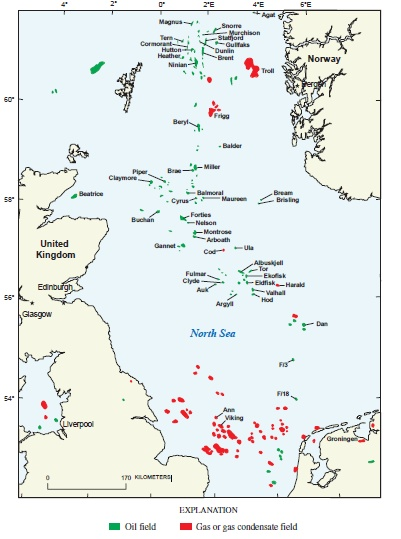
\includegraphics[scale=0.7]{northseaoilandgasmap}
	\caption{Map of oil and gas fields in the North sea}
	\todo[inline]{Get higher resolution picture}
	\label{fig:northseamap}
\end{figure}

% More recently, offshore wind energy and the oil and gas industry have  offshore structures typically located on continental shelves some miles off the coast. 


%Recently, developments in the oil and gas industry have necessitated extensive use of specialised vessels called offshore supply vessels in aid of exploration and production operations. These 

%the construction and maintenance of offshore oil platforms typically located in continental shelves. 

Handling vessels at low speeds has been difficult on marine vessels historically. From a technical point of view, the working mechanism of rudder systems of the past made it difficult to turn vessels in place. From a human operator perspective, the challenge of maneuvering at low speed is further amplified when the operation occurs in close proximity to large physical objects due to the added stress from the risk of collision. Refer to \citep{inoue2000evaluation} for a method of objective evaluation of ship handling difficulties in restricted maneuvering area or in areas of traffic congestion. Examples of difficult maneuvering operations are approaching a harbour, berthing in a port, sailing side-by-side another vessel, approaching and stationing close to an oil platform, etc. An often recurring sequence is that of  port-bound vessel heading to its berthing location in the harbour. Having entered pilot waters from seaward, a vessel's course needs to be controlled to ensure safe passage through channels, bridges, and locks; while avoiding collisions with other vessels at the same time. Safety risks involved in such tasks make it a stressful operation. Mistakes have high associated costs, possibly leading to lost lives and damage to expensive constructions.


% Mistakes in execution have high costs associated with them as they can lead to lost lives and damage to expensive constructions. 

%Executing a maneuvering operation in close proximity to large man-made physical structures is particularly challenging. the added stress due to risk of collision makes the task particularly challenging. 
%A maneuvering operation that takes place in close prox

A special application of ship handling skill is on-board offshore supply vessels. Offshore supply vessels are cargo vessels that regularly transport goods, supplies or equipment in support of exploration or production of offshore mineral or energy resources. Specific missions include: 
\begin{itemize}[noitemsep]
\item seismic survey to locate potential oil and gas fields
\item towing of rigs to their location, positioning them and laying anchoring and mooring equipment
\item supplying equipment, personnel, provisions, other necessary goods to rigs
\item subsea operations such as ROV operation, diving support, inspection and maintenance
\item safety standby for emergency response and rescue operations
\end{itemize}
 Offshore supply vessels need to regularly approach and be stationed close to offshore oil platforms to perform supply operations. A platform supply vessel for example, is used to transport supplies such as fuel, water and chemicals to oil platforms; bringing back disposables for proper recycling. 
\begin{figure}[hb]
	\centering
	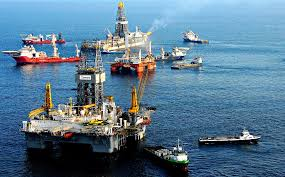
\includegraphics{osvbig}
	\caption{Offshore supply vessels in operation}
	\label{fig:shipforces}
\end{figure}

A typical loading operation happens at the stern of the ship. requires station keeping.


This requirement led to the development and subsequent popularity of dynamic positioning systems. Dynamic positioning (DP) is a computer-controlled system that maintains position and heading of a vessel automatically by using its propellers and thrusters. Information from position reference sensors that provide the vessel’s position and heading, along with information from wind sensors, motion sensors and gyrocompasses on the vessel are used by the system. The information is supplied as input to a program that calculates the changes in position/heading required to bring the vessel a preset location and, activates the vessel’s thrusters as necessary.

\begin{figure}
	\centering
	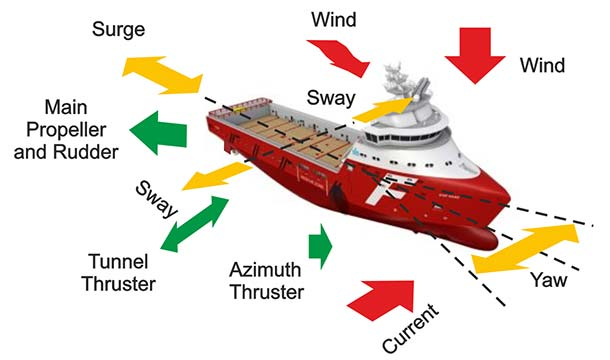
\includegraphics[scale=0.60]{dynamic-positioning}
	\caption{Forces acting on a ship and its possible movements}
	\label{fig:shipforces}
\end{figure}
\missingfigure{Make a sketch of the forces on a ship and its movements}
\todo[inline]{make own picture with legend of forces}
%Write about the popularity of Dp systems, its advantages and disadvantages. Mention increasing automation and the need for manual control ability. 

The use of dp systems has been increasing over the years since its first inception in 1960s. There are well over 2000 DP vessels in operation today \citep{sorensen2011survey}. From the early days of the technology where main focus areas of research were accurate position measurement and control system technologies used, research has now moved on to more specialized problems such as optimizing dp systems for energy efficiency. With increasing popularity of DP systems and increased use of sophisticated technology onboard ships, the marine industry can expect more advanced automation in vessel control over the years. Future systems could be enabled with features such as automatic maneuvering in shallow water and harbor areas, formation sailing, and automatic collision avoidance.

%The popularity of DP systems has grown to a point where they are a component of medium to large sized vessels these days. 

%This evolution of navigation technology on ships from mere position monitoring systems to automatic position control system has been accompanied by a corresponding growth of specialized personnel responsible for the monitoring of DP systems. 

%From PID to Advanced Control The first DP systems introduced in the early 1960s used conventional PID controllers in cascade with low-pass and/or notch filters to suppress the first-order wave-induced motion components. From the mid-1970s, more advanced control techniques were proposed based on linear optimal control and Kalman filter theory. With improvements and increasing sophistication in vessel control, the marine industry can look forward to more advanced control features such as DP-assisted position mooring systems, automatic maneuvering in shallow water and harbor areas, formation sailing, and automatic collision avoidance. These applications open new possibilities for the expansion of functionality in DP systems.

Dynamic positioning is an automated system that helps human operators with maneuvering operations. It offloads part of the human operator's decision making overhead in real-time. Using a mathematical model of the ship and, the forces acting on it, the DP system can control the vessel's thrusters to position it in a preset destination. Figure \ref{fig:dparchitecture} is a model of the functional components of a dynamic positioning system. 
\begin{figure}
	\centering
	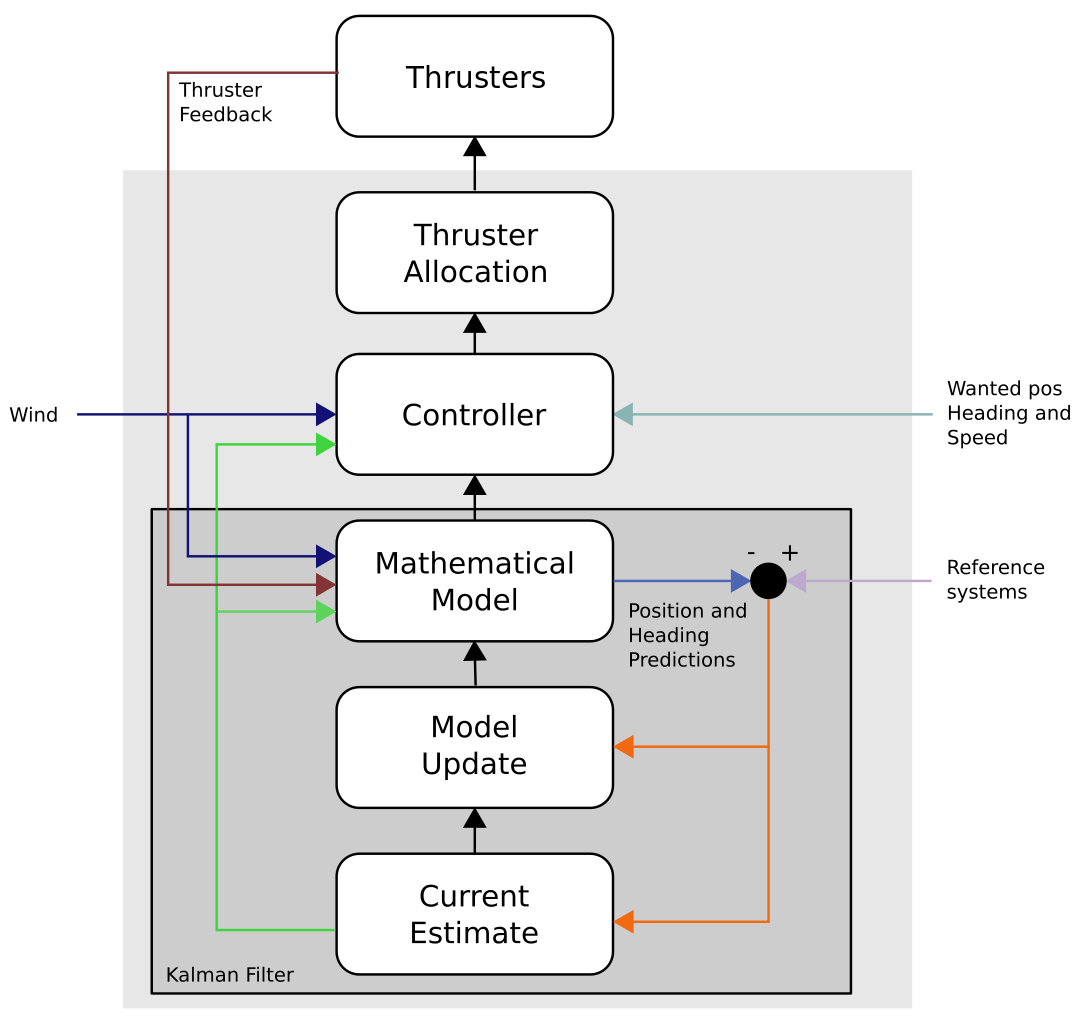
\includegraphics[scale=0.25]{dparchitecture}
	\caption{Model architecture of Dynamic Positioning systems}
	\label{fig:dparchitecture}
\end{figure}


The system contains a \textit{controller} module that influences vessel movements by taking decisions on power allocation for individual vessel thrusters. It takes as input, weather information from wind sensors and current position information from position reference systems. Expected output is to position the vessel at a position and heading preset by the operator. After being initiated, the system determines the difference between current position and desired position. It then attempts to minimize this difference over time. This is done by firing appropriate thrusters into action, producing vessel movements in different directions. 

Environmental forces acting on the vessel during the time though add to the complexity of this operation. The controller then needs to compensate for unpredictable environmental forces as it decides on allocations for individual thrusters.  While the system takes into account wind forces acting on the vessel measured using wind sensors, as shown in \ref{fig:shipforces}, a vessel's position is also affected by ocean currents and waves. Kalman filter is generally used to model the environmental forces. It is an algorithm that uses a series of measurements observed over time, containing statistical noise and other inaccuracies, and produces estimates of unknown variables by using Bayesian inference and estimating a joint probability distribution over the variables for each timeframe. While it tends to be more precise than algorithms based on a single measurement alone, it is a nevertheless a probability based system that produces estimate predictions of changes in environmental forces over time and some uncertainty in predictions can be expected. Although there do not exist rules specifying acceptance criteria for the positioning performance of DP systems, DNVGL guidelines state that "in moderate weather conditions and with a fully operational DP-system the vessel should generally be able to demonstrate position keeping accuracy with a 3 meter radius and ± 1° of heading." \citep{veritas2011dynamic} 

\todo[inline]{write about accidents that occured. ekofisk etc}

Figure \ref{fig:praxisdp} shows the interface of a typical DP system. A display monitor is used to show various information regarding the vessel and its control systems. Apart from the display, there exists input interface in the form of buttons. They are used to provide information to the system such as desired location and the mode in which it will be used. Modes here refer to the various types of automatic vessel operation that differ in the amount of automation involved. Some of the common modes of operation are listed below. 

\begin{figure}
	\centering
	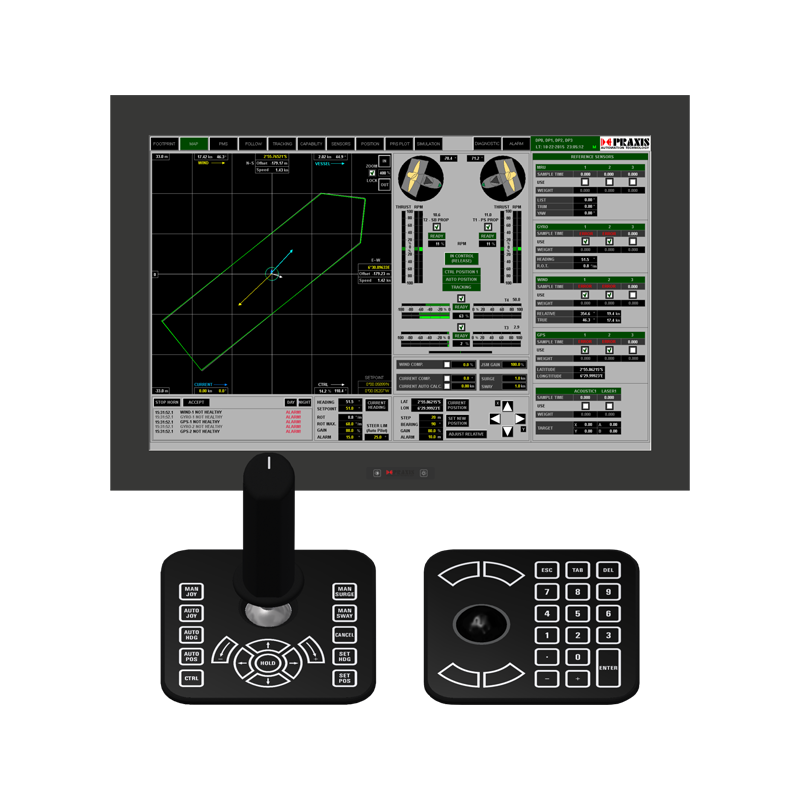
\includegraphics[scale=1]{praxisdp}
	\caption{Typical dynamic positioning console}
	\label{fig:praxisdp}
\end{figure}

\begin{enumerate}

\item \textbf{Joystick}: In this mode, the operator can control the vessel position and heading manually using a joystick. 
\item \textbf{Auto heading}: In this mode, the vessel automatically maintains a preset heading. 
\item \textbf{Auto position}: This mode automatically maintains the vessel's position and heading. 
\item \textbf{Follow target}: Enables the vessel to automatically follow a moving target. 
\item \textbf{Autopilot}: In this mode, the vessel steers automatically to follow a predefined course. 

\end{enumerate}

This is by no means an exhaustive list of DP modes. It can be noted that besides functionality, the modes listed above differ by the level of automation involved in the functionality.  The joystick mode offers the least amount of automation. In this mode, a single lever can be used to control all of the vessel's thrusters at the same time. A large vessel such as a platform supply vessel typically has two azimuth thrusters at the stern-end of the vessel and one at the bow-end. In addition, they also typically have tunnel bow thrusters that can be used to turn the vessel in place. While it is possible to control each of the thrusters individually from the bridge of the vessel for fine-grained control; the joystick mode encapsulates all the thrusters into one control. This allows the captain to control forward, reverse, steering and even sideways motion using just one lever.

\missingfigure{insert layout of typical PSV thrusters}

\begin{figure}
	\centering
	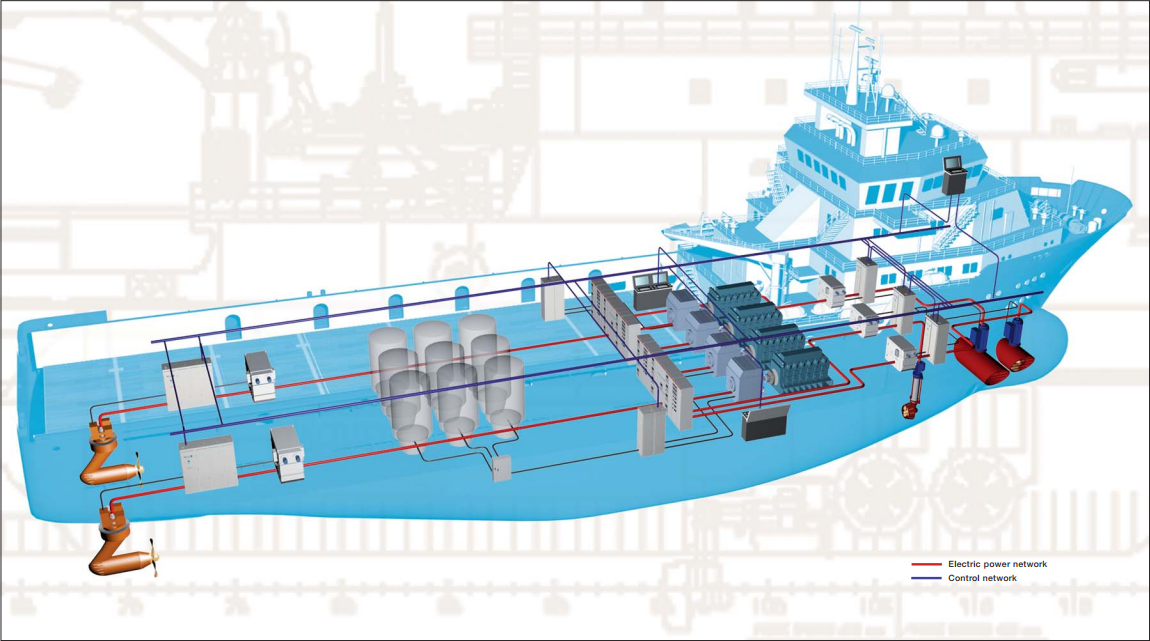
\includegraphics[scale=0.25]{osvlayout}
	\caption{Schematic diagram of the power and control network of a typical offshore supply vessel}
	\label{fig:osvlayout}
\end{figure}

Going by number of total losses occuring per year (refer figure \ref{fig:lossesbyyear}), the safety of vessels world-wide can be said to have improved over the years, particularly the last decade, despite the ever increasing number of sea-faring vessels. Nevertheless, there is a growing concern in the industry regarding overreliance on electronic navigation aids. Studies have found human error to be dominant factor in a significant percentage of the accidents \citep{baker2005accident, hauff2014analysis}. Incidents such as the Norne shuttle tanker's collision with an FPSO on 5 March 2000, Big Orange XVIII's collision with the water injection facility Ekofisk 2/4-W on 8 June 2009 and standby vessel Far Symphony's impact with the mobile installation West Venture on 7 March 2004 are mentioned as cases of shipping incidents that showcase the lack of preparedness among crew members to handle with emergency situations \citep{vinnem2013offshore}.

\begin{figure}
	\centering
	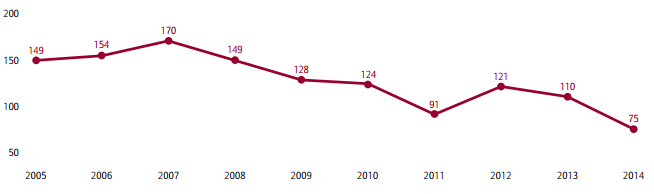
\includegraphics[scale=0.75]{lossesbyyear}
	\caption{Schematic diagram of the power and control network of a typical offshore supply vessel}
	\label{fig:lossesbyyear}
\end{figure}


